Dans cette section, nous vous présentons le prototype graphique.

\subsection{Menu principal}
Voici le menu principal, depuis celui-ci, il sera possible de jouer, de paramétrer le jeu, de quitter le jeu ou alors de gérer le jeu.
\begin{figure}[ht]
	\centering
	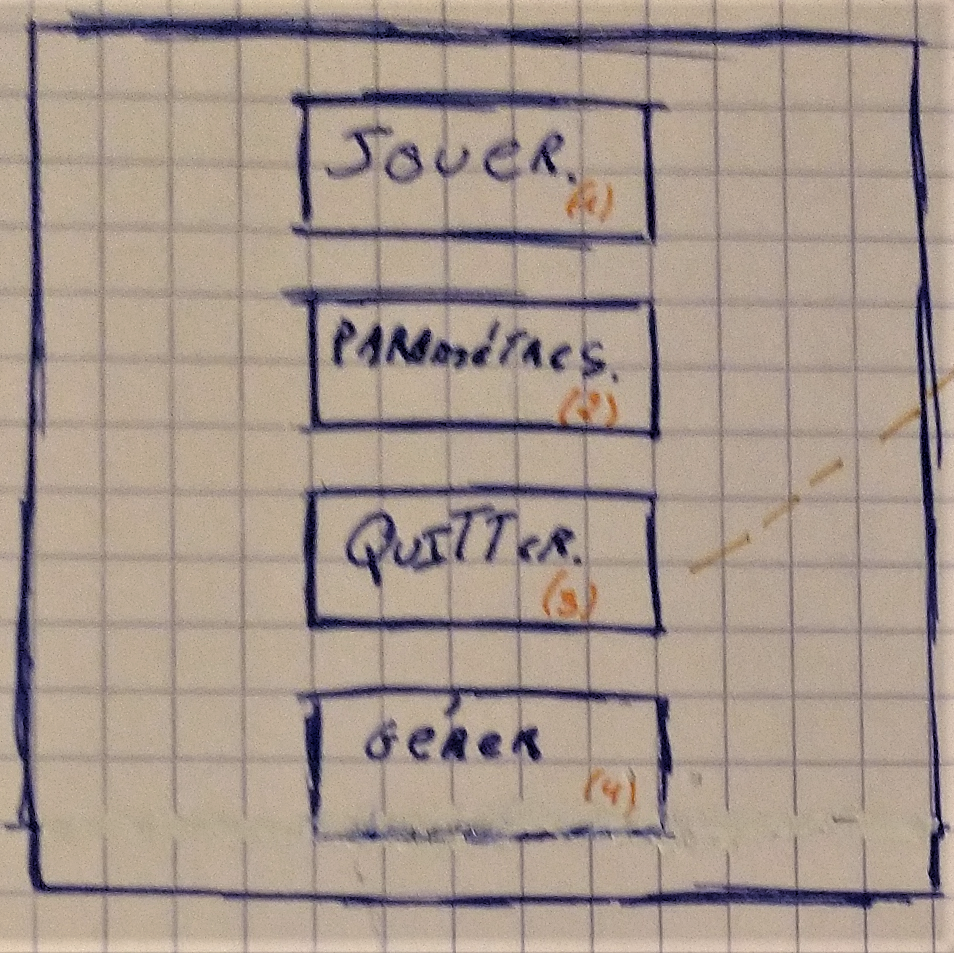
\includegraphics[scale=0.5]{menu_principal.png}
	\caption{menu principal}
	\label{interface menu}
\end{figure}

\newpage
\subsection{Menu joueur}
Le menu joueur sera un combo de label et de textfield, il sert à prendre des informations sur le nom des équipes. Il faut au minimum deux équipes ou joueurs.
\begin{figure}[ht]
	\centering
	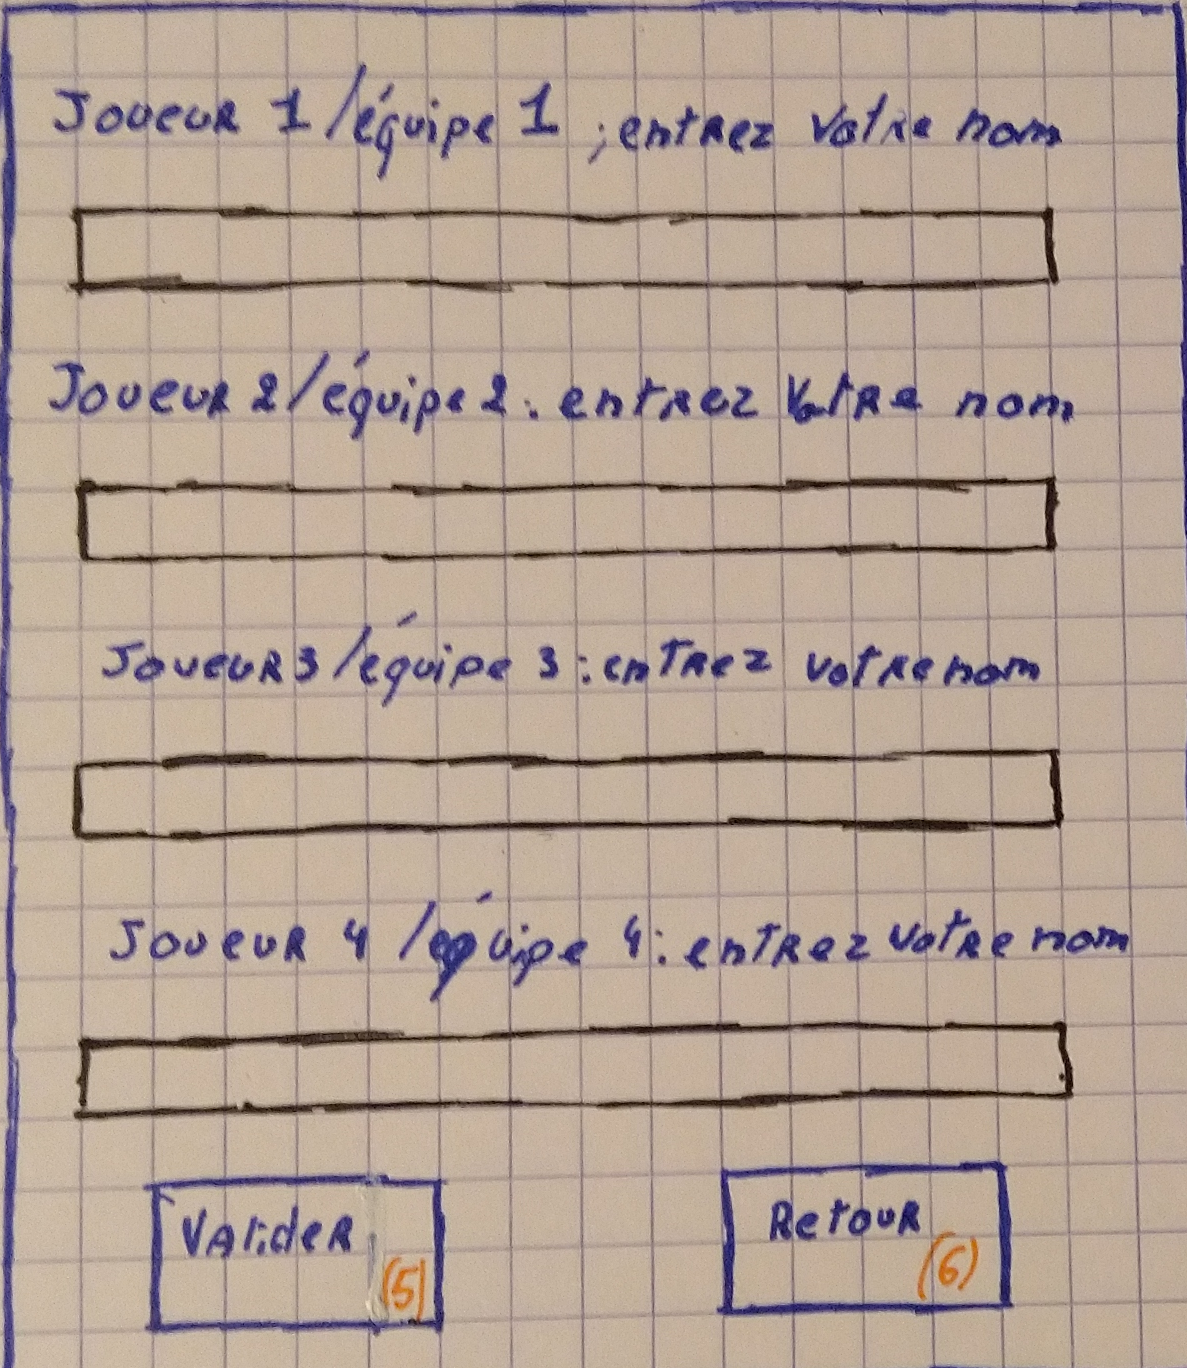
\includegraphics[scale=0.5]{menu_joueur.png}
	\caption{nom des joueurs ou équipe}
	\label{interface création d'équipe}
\end{figure} 

\newpage
\subsection{Fênetre erreur du nombre de joueurs}
Dans le cas où l'on n'entre pas suffisamment de joueur ou d'équipe, une alerte va notifier le joueur qu'il n'y a pas assez de joueur et ne peut donc pas jouer dans que cela n'est pas réglé.
\begin{figure}[ht]
	\centering
	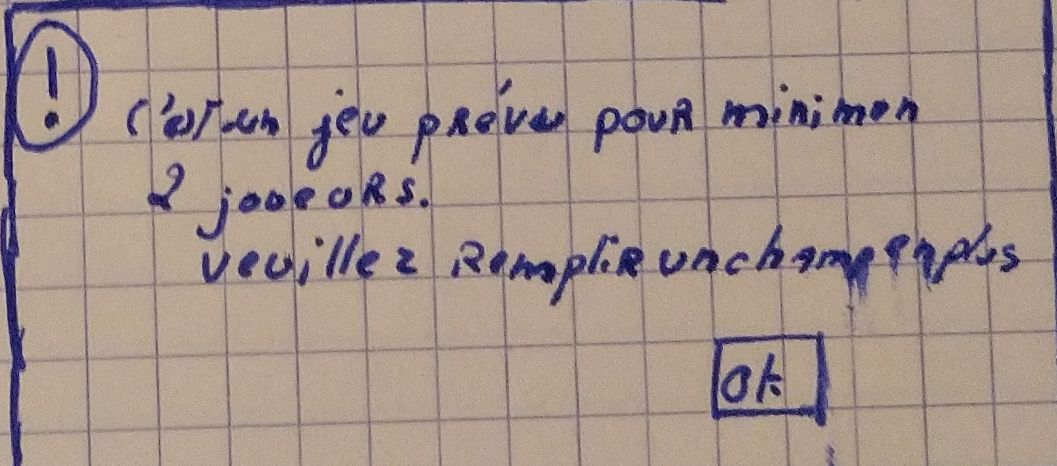
\includegraphics[scale=0.5]{fenetre_erreur_nb_joueur.png}
	\caption{alerte de non conformité du nombre de joueurs}
	\label{alerte du nombre de joueurs}
\end{figure}

\newpage
\subsection{Jeu}
Le UI sera composé d'un label avec le nom de l'équipe, un autre avec un des quatre thèmes, et un dernier avec le sujet de la question. Ensuite, il y a quatre boutons cliquable avec un numéro de un à quatre. Le numéro sur le bouton correspond 
à la difficulté de la question par ordre croissant.
\begin{figure}[ht]
	\centering
	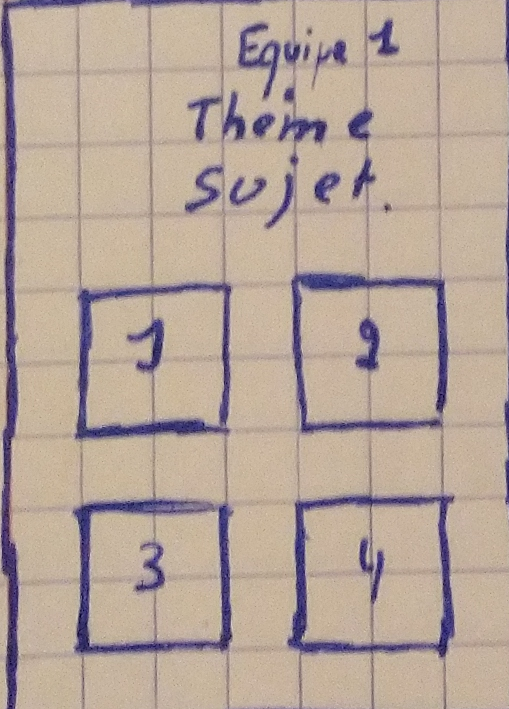
\includegraphics[scale=0.5]{jeux.png}
	\caption{choix de la difficulté de la question}
	\label{interface jeu}
\end{figure}

\newpage
\subsection{Fênetre quitter}
Il s'agit d'une fênetre permettant de vérifier si le joueur veux réellement quitter la partie. Cette fênetre est composer d'un label et de deux boutons permettant soit de quitter l'application, soit de retourner au menu principal.
\begin{figure}[ht]
	\centering
	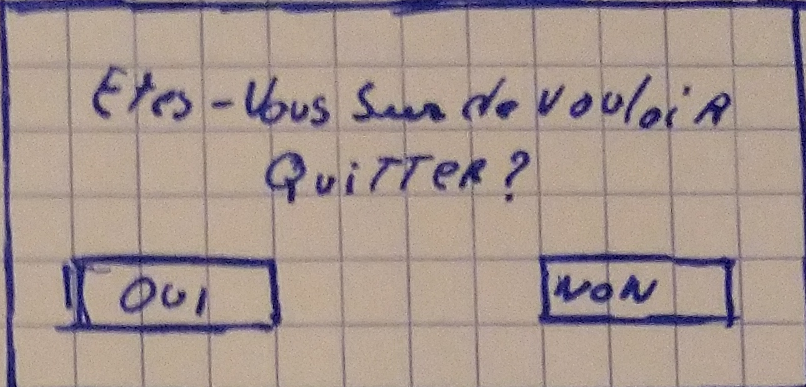
\includegraphics[scale=0.5]{fenetre_quitter.png}
	\caption{fêntre pour quitter le jeu}
	\label{fênetre pour quitter le jeu}
\end{figure} 
